%\frame{\titlepage}

\section{Kommunikation}

%\frame{\tableofcontents}
%\section{Einleitung}

\subsection{Einleitung}
%\frame
%{
%  \frametitle{Einleitung}
%  \begin{itemize}
%    \item Zur Koordination haben die NAOs die M\"oglichkeit, miteinander zu kommunizieren.
%  \end{itemize}
%  %\begin{center}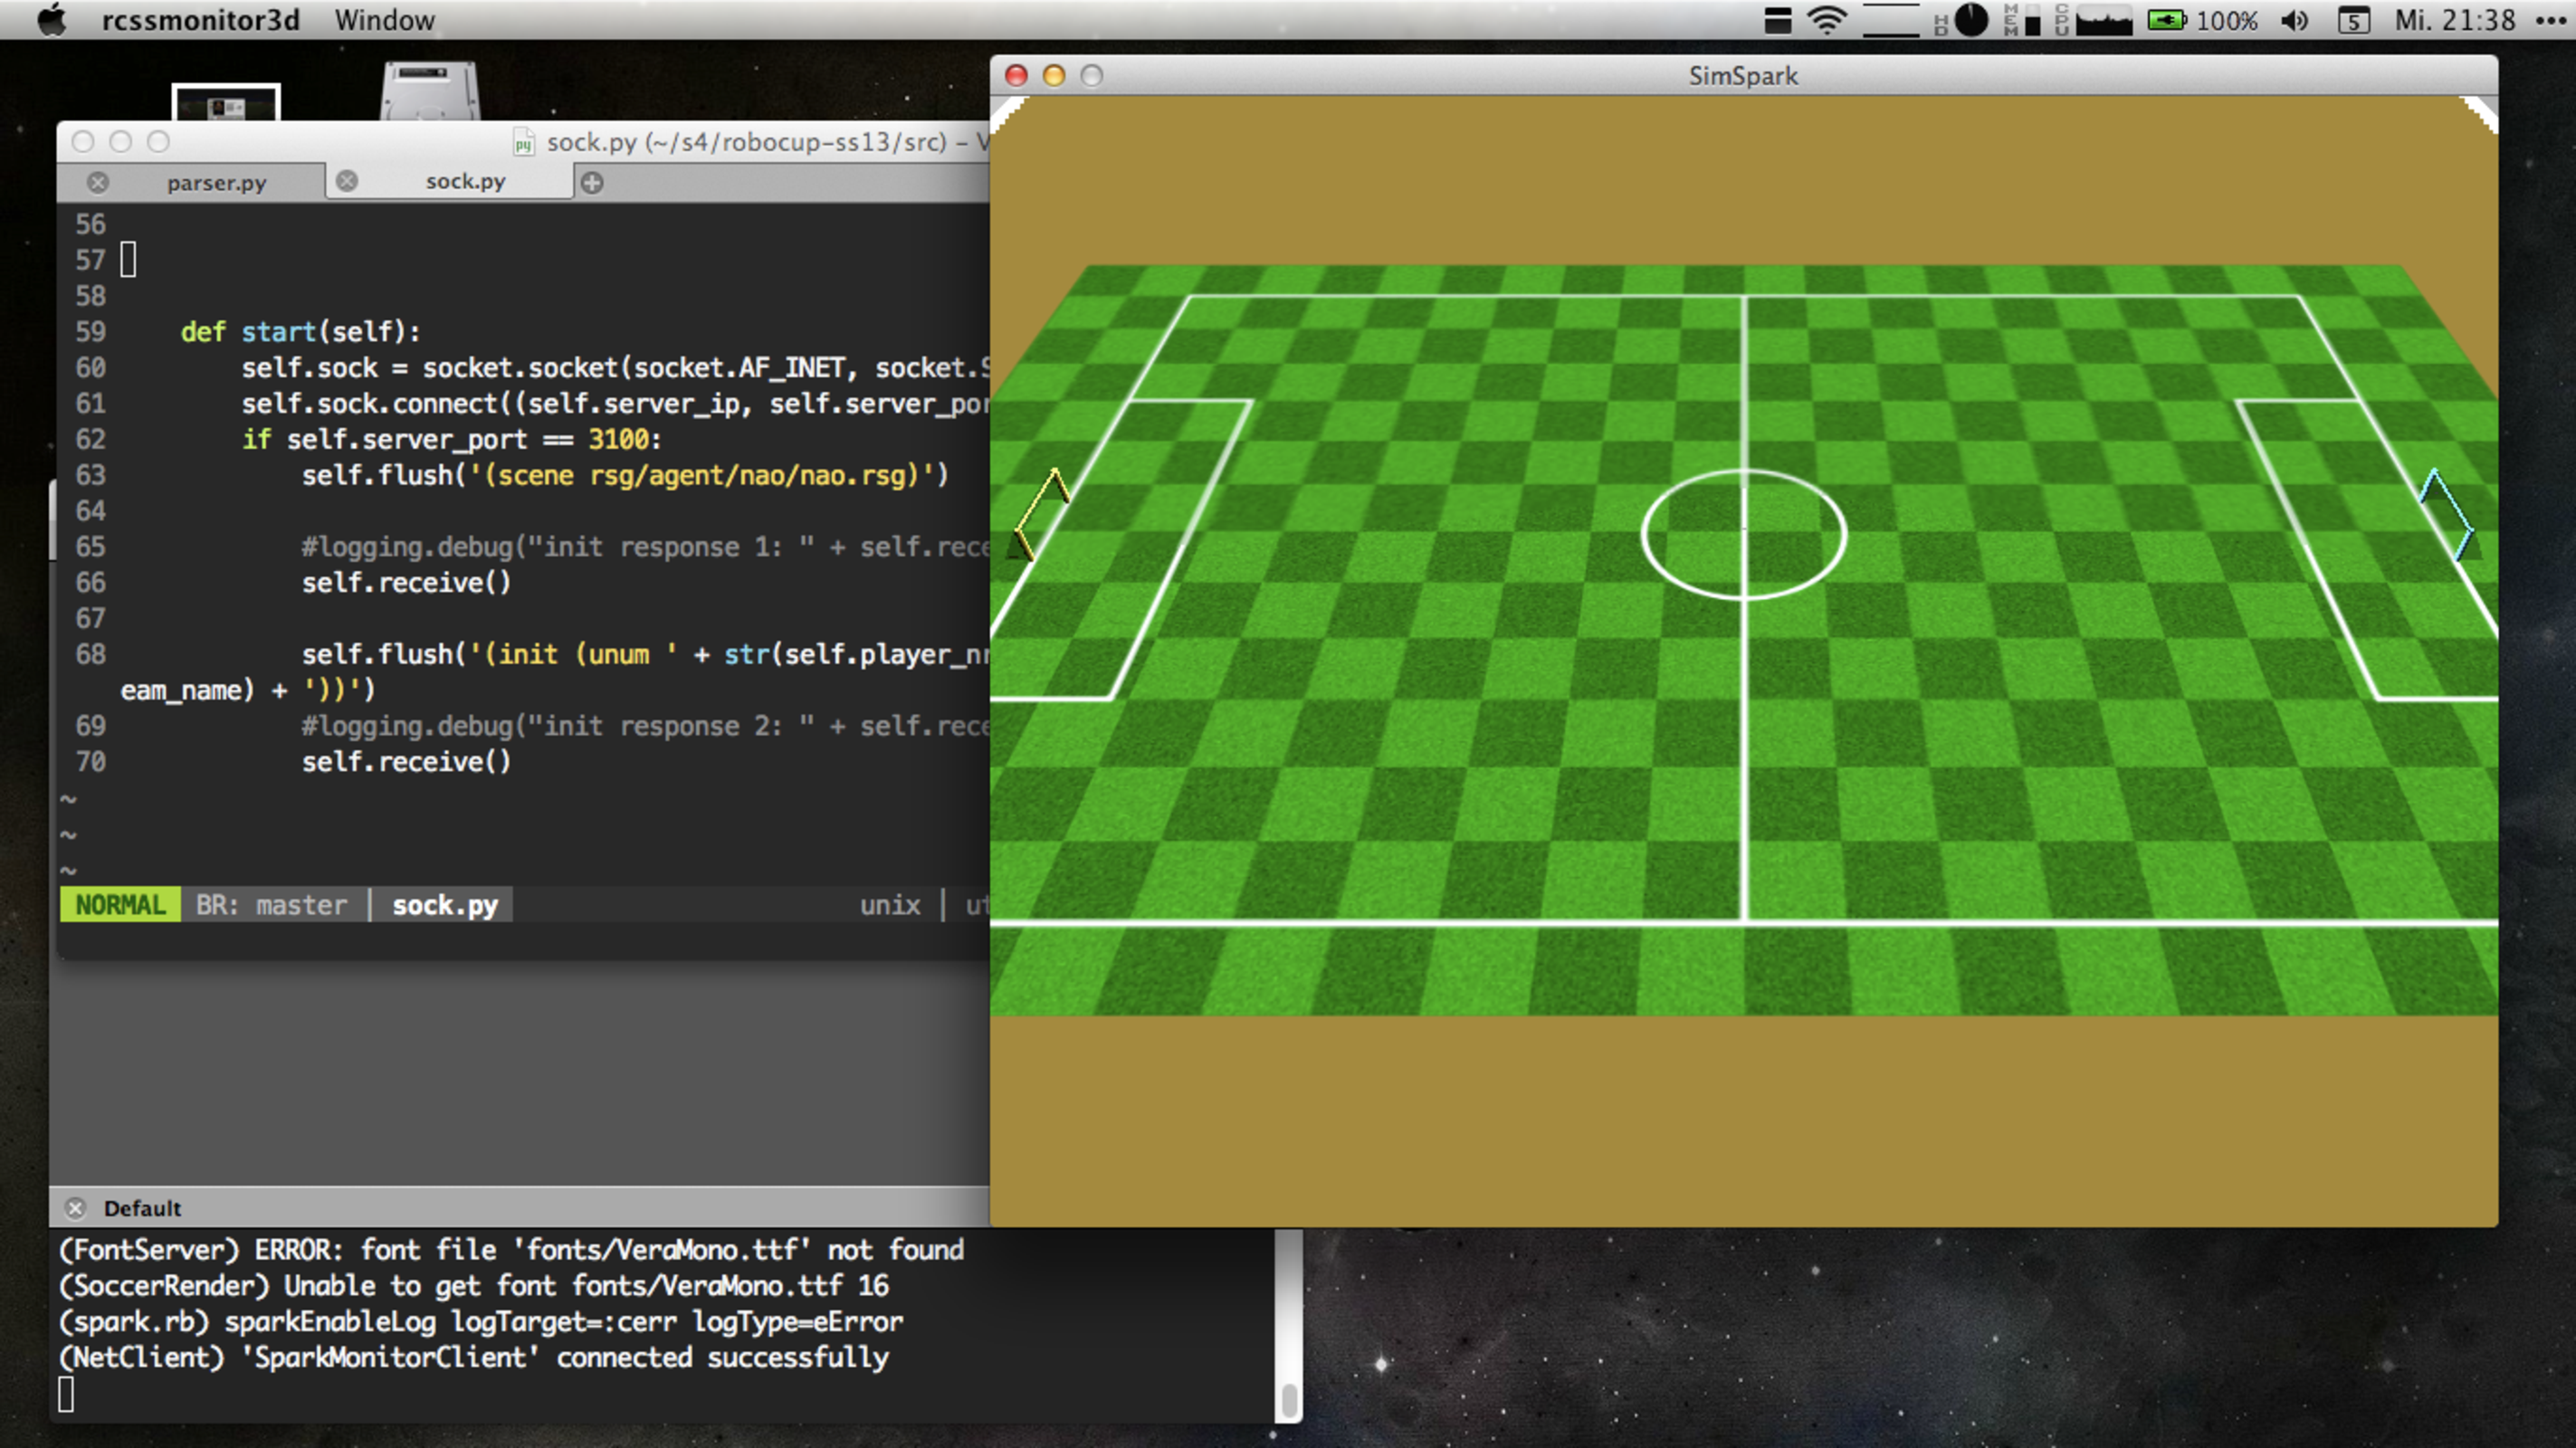
\includegraphics[height=5cm, center]{simulator.pdf}\end{center}
%}
  
\frame
{
  \frametitle{Einleitung}
  \begin{itemize}
    \item Das funktioniert, im Prinzip, wie bei Menschen auch:
    \item Zun\"achst wird die Nachricht erstellt und codiert.
    \item \"Uber den Server wird sie nun an die NAOs weitergeleitet.
    \item Diese m\"ussen die Nachricht entschl\"usseln und interpretieren.
  \end{itemize}
  
  \begin{center}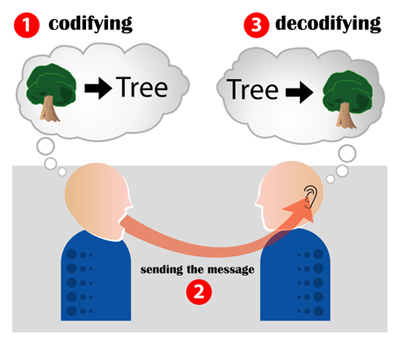
\includegraphics[height=5cm, center]{Encoding_communication.jpg}\end{center}
}

\frame
{
  \frametitle{Die Rahmenbedingungen}
  \begin{itemize}
    \item Die Kommunikation unterliegt einigen Einschr\"ankungen: \vskip0.3cm
    \item Maximal 20 Zeichen pro Nachricht.
    \item Es steht nur ein eingeschr\"ankter ASCII-Zeichensatz zur Verf\"ugung. (90 Zeichen)
%    \item Es gibt noch einige weitere Einschr\"ankungen der Kommunikation, die zu beachten sind: \vskip0.5cm
    \item Ein NAO ist 50m weit zu h\"oren.
    \item Er kann ausserdem nur alle 0.04s etwas h\"oren. In der Zwischenzeit kann er keine Nachrichten empfangen.
    \item Sollten 2 NAOs gleichzeitig sprechen, wird nur einer von ihnen geh\"ort. Der Sprecher h\"ort sich jedoch immer selbst.
    \item Die Teams sprechen versetzt, man kann also nicht die Kommunikation des anderen Teams blockieren.
  \end{itemize}
}

\subsection{Codierung}
%\section{Parser}
\frame
{
  \frametitle{Codierung}
  
  \begin{itemize}
    \item \"Uber say-Methoden kann eine Nachricht codiert werden.
    \item Eine codierte Nachricht ist wie folgt aufgebaut: \vskip0.5cm
    \item $<MessageCode><Parameter><Pr\ddot{u}fsumme>$ \vskip0.5cm
    \item Ein Message-Code definiert hier die Art der Nachricht.
    \item Sender, Empf\"anger und Parameter sind dahinter angeh\"angt. \\Doubles als Parameter haben einen Wertebereich von $\pm$364.00.
    \item Am Ende wird die Nachricht durch eine Pr\"ufsumme validiert.
  \end{itemize}
}

%\subsection{Senden und Empfangen}
%%\section{Probleme}
%\frame
%{
%  \frametitle{Senden der Nachricht}
%  
%  \begin{itemize}
%    \item Nachdem die Nachricht codiert ist, kann sie versendet werden.
%    \item Hierzu steht einem der Say-Effector des NAO zur Verf\"ugung.
%    \item \"Uber ihn gelangt die Nachricht an den Server.
%  \end{itemize}
%}
%
%\frame
%{
%  \frametitle{Empfangen der Nachricht}
%  
%  \begin{itemize}
%    \item Nun muss die Nachricht nat\"urlich auch empfangen werden.
%    \item Daf\"ur nutzen wir den Hear-Perceptor des NAO.
%    \item Wenn der NAO gerade zuh\"ort, empf\"angt er \"uber ihn die Nachricht.
%    \item Hierf\"ur steht eine Methode hear(...) zur Verf\"ugung.
%  \end{itemize}
%}

\subsection{Decodierung}
\frame
{
  \frametitle{Decodierung}
  
  \begin{itemize}
    \item Zun\"achst wird die Nachricht von einem Translator in ihre Bestandteile aufgetrennt.
    \item Daraus wird ein HearObject erstellt.
    \item Dieses unterscheidet sich je nach Nachricht, und alle relevanten Daten sind in ihm gespeichert.
    \item \"Uber eine eval()-Methode kann das Objekt nun ausgewertet werden. (Taktik)
  \end{itemize}
}

%\subsection{Fazit}
%\frame
%{
%  \frametitle{Weitere Details}
%  
%  \begin{itemize}
%    \item Es gibt noch einige weitere Einschr\"ankungen der Kommunikation, die zu beachten sind: \vskip0.5cm
%    \item Ein NAO ist 50m weit zu h\"oren.
%    \item Er kann ausserdem nur alle 0.04s etwas h\"oren. In der Zwischenzeit kann er keine Nachrichten empfangen.
%    \item Sollten 2 NAOs gleichzeitig sprechen, wird nur einer von ihnen geh\"ort. Der Sprecher h\"ort sich jedoch immer selbst.
%    \item Die Teams sprechen versetzt, man kann also nicht die Kommunikation des anderen Teams blockieren.
%  \end{itemize}
%}

%\frame
%{
%  \frametitle{Zusammenfassung}
%
%  \begin{itemize}
%    \item Communication.py stellt Methoden zur Kommunikation zur Verf\"ugung.
%    \item say-Methoden dienen dem senden von Nachrichten.
%    \item Soll der NAO zuh\"oren was gesagt wird, benutzt man hear().
%    \item Man erh\"alt nun ein HearObject.
%    \item \"Uber eval() wertet man es zu einem geeigneten Zeitpunkt aus.
%  \end{itemize}
%}